\documentclass{article}
\usepackage{graphicx}
\usepackage{latexsym}
\usepackage[french]{babel}
\usepackage[utf8]{inputenc}
\usepackage[T1]{fontenc}
\usepackage{listings}

\title{Rapport du projet C++ : Lancer de rayons}
\author{Mathieu \textsc{Mari} \and Xavier \textsc{Montillet}}

\begin{document}

\title
\tableofcontents
	

\section{Introduction}
Dans ce nouveau projet, nous nous sommes intéressé à la technique du lancer de rayons et nous l'avons implémenter en C++.
Cette technique permet de générer des images 3D à partir de la déscription des objets présent dans la scène ainsi que de la position de la caméra. Elle a son utilité dans les logiciels d'images de synthèse, la création de jeux vidéos, la simulation numérique\dots  	

\section{Implémentation en C++}
	\subsection{Principe général}
	\paragraph{}		
Afin de générer l'image 3D d'une scène, il faut deja définir quels sont les objets qui composent la scène, c'est dire définir quel est leur type (sphère, plan, \dots), quelle est leur position, leur couleur, leur texture\dots. Ensuite, il faut choisir la posistion des sources lumineuses puis leur couleur, leur intensité\dots Enfin, il faut positionner la caméra qui observe la scène. Pour cela, on choisit un point qui sera la position de l'objectif, puis la position de l'ecran sur lequel l'image sera projetée.

	\paragraph{}
		Fabriquer une image, c'est calculer pour chaque pixel sa couleur. Dans cette optique, le principe de la technique du lancer de rayons consiste à créer une demi-droite ayant pour origine l'objectif de la caméra et passant par le un pixel de l'écran. On regarde quel objet de la scène est intersecté en premier par la demi-droite. On calcule ensuite la couleur du pixel en regardant combien de sources éclairent le point d'intersection entre la demi-droite et l'objet, quel est la couleur de l'objet et des sources, est-ce qu'il y a reflection, refraction, transparence\dots

		\subsection{Les différentes classes utilisées}

Afin de représenter les différents éléments qui seront nécessaires à la technique du lancer de rayons et leur dépendance mutuelle, nous allons utiliser les classes C++.
Le schéma de dépendance des classes est le suivant :
	\begin{center}
    		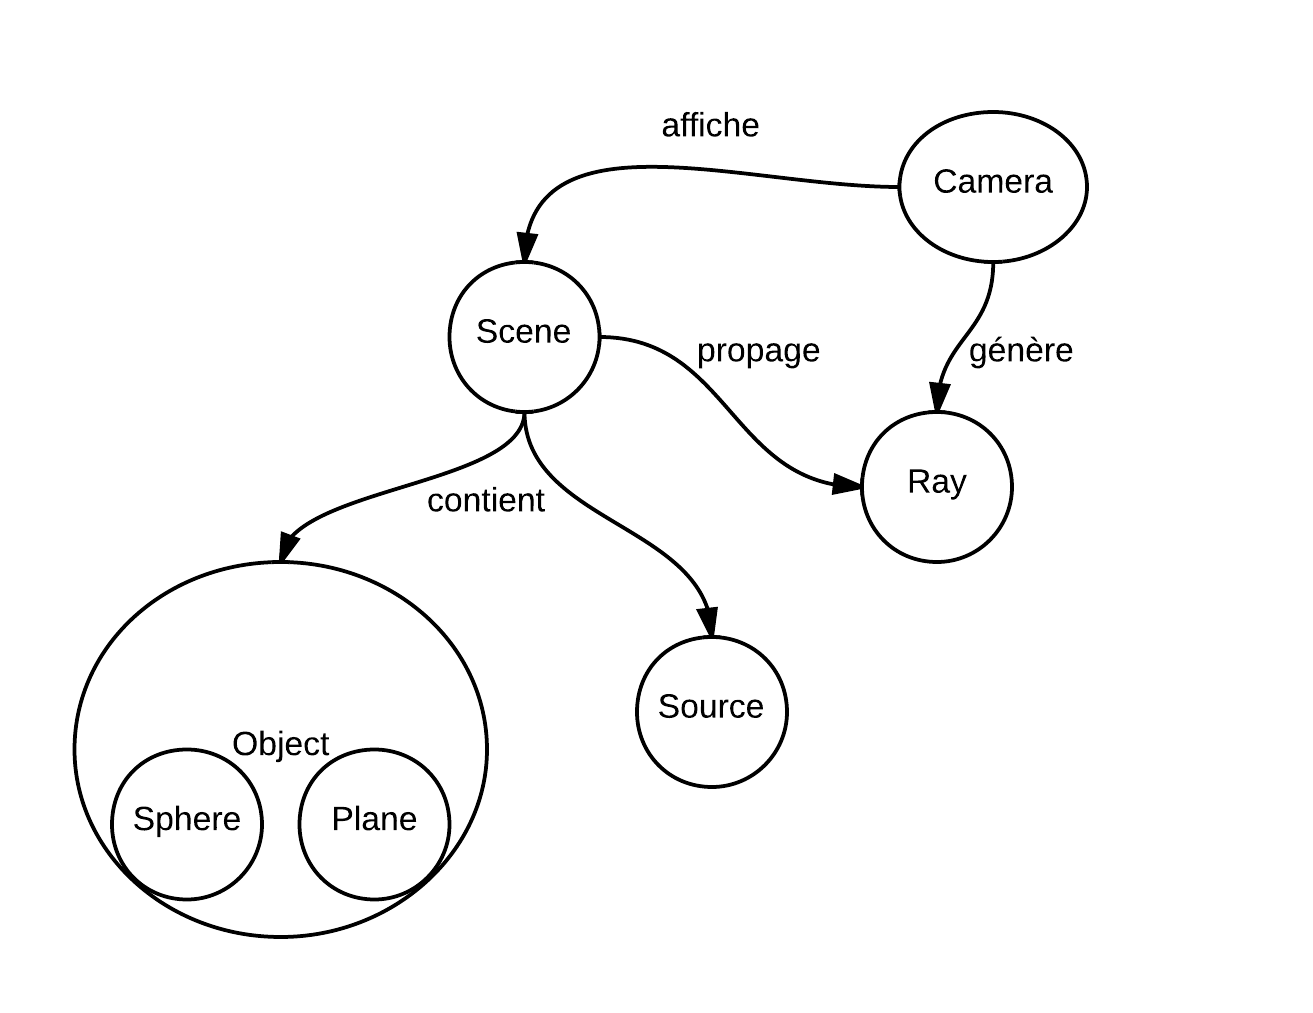
\includegraphics[height = 7cm]{schema.png}
  		\end{center}



\end{document}
